\chapter{Calibration}

Our goal is to create a system which does not need any prior information about the
position of cameras. Since we do not know how far away the cameras are, nor
angles between them, we firstly use calibration to obtain this information.

By calibrating cameras with a well describable pattern, we can obtain
information about the single camera, such as what distortion its lens cause, or
how the world points are projected to an image plane of the camera.

After discovering these parameters for both cameras, we will continue on stereo
calibration. Stereo calibration will provide us information about their
position in space relative to each other.

For these calibration processes, we use algorithms implemented in OpenCV.
Therefore, we provide only a short overview of the process, and we describe
only results obtained from calibration essential to us.

\section{Intrinsic parameters}

Each camera type is different. Moreover, each camera of a specific type is
different due to a manufacturing process. Therefore we introduce intrinsic
camera parameters, which help us to model the camera precisely.

Intrinsic camera parameters define a transformation between the world coordinates and
the coordinates within an image plane (in pixels). Physical attributes of the
camera influence this transformation.

These parameters include focal length, a position of the principal point and
distortion coefficients. All these parameters are needed to get a correct
transformation between the point in the space and the point at the image plane.
Sometimes even more parameters are used for a better description of the model
of the camera.

\subsection{Camera matrix} 

Camera matrix will provide us a transformation from
world coordinates (with the origin in the camera) to image plane coordinates
(seen in the image taken from the camera). If the coordinates in 3D are
available, we can obtain 2D coordinates by simple multiplication by camera
matrix. After multiplication we obtain 2D homogeneous coordinates.

As the next step, we describe the camera matrix obtained by OpenCV calibration
procedure. In the OpenCV implementation the camera matrix is $3\times3$ matrix of the
following format:

\[
\begin{pmatrix}
	f_x 	& 0 	& c_x \\
	0	& f_y	& c_y \\
	0	& 0	& 1
\end{pmatrix}
\]

Where $f_x$, $f_y$ denote focal lengths expressed in pixel units. It is usual
to introduce two of them, separately for both axes, since pixels usually are
not perfect squares but rather rectangles. Therefore the same focal length, has
different length in pixel units over a given axis.

We refer the ray of the view of the camera as the principal ray. The point
where this ray intersects the image plane is called principal
point\footnote{For more information visit \url{https://en.wikipedia.org/wiki/Pinhole\_camera\_model\#The\_geometry\_and\_mathematics\_of\_the\_pinhole\_camera}}.
Parameters $c_x$ and $c_y$ define coordinates of the principal point in the
image plane.  It should be the center of the image, but assembling process of
the camera might cause a small displacement.

\subsection{Distortion coefficients}

Cameras are equipped with lenses to obtain sharp image instead of blurry. The
lens may causes various distortions. Fish-Eye lenses are known for their
distortion.  Even web camera lenses have distortion, but not as visible as the
camera with a fish-eye lens. It is important to correct these distortions.

Two distortion types cause a significant effect on the image. The first one is
the radial distortion, creating barrel effect and the second one tangential distortion.

The radial distortion is caused by the camera lens (the effect of radial
distortion is displayed in the image \ref{fig:distortion}). It can usually be
described by three parameters. Highly distorted images (like from fish-eye)
often need more parameters. Since our system use web cameras, we will use only
three parameters.

In the ideal camera, the lens would be placed parallel to the chip. Since such
precision is not possible, due to an assembling process, tangential distortion
arises. For this distortion, we use two parameters.

We describe both distortion effects by five parameters. More about the meaning
of the parameters could be found in the book by \citet*{bradski2008learning}.

\begin{figure}
	\begin{subfigure}[b]{0.48\linewidth}
		
\includegraphics[width=\linewidth]{img/chessboard/7x8chessboard-positivedistortion}
		\caption{Effect of positive radial distortion}
	\end{subfigure}
	\begin{subfigure}[b]{0.48\linewidth}
		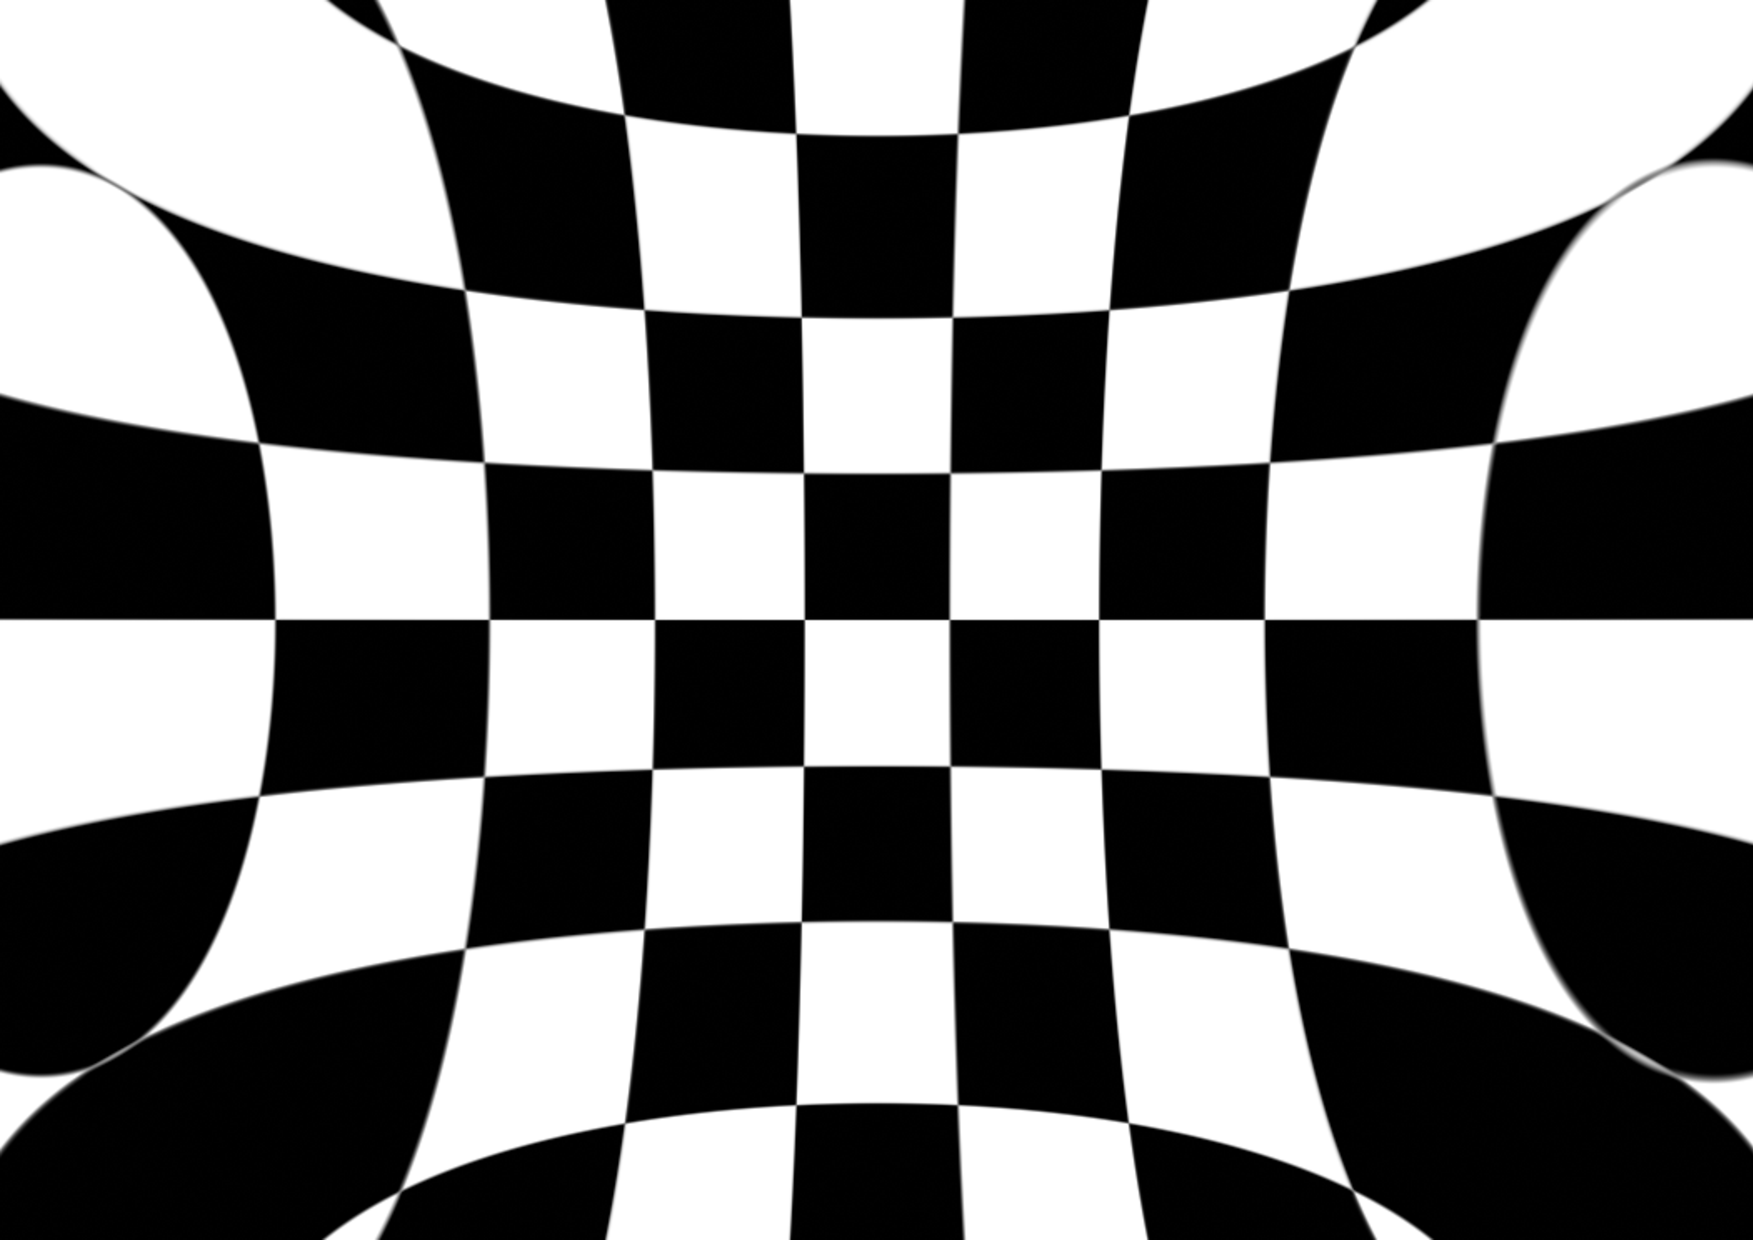
\includegraphics[width=\linewidth]{img/chessboard/7x8chessboard-negativedistortion}
		\caption{Effect of negative radial distortion}
	\end{subfigure}
	\caption{Effects of lens distortion on the image of the chessboard}
	\label{fig:distortion}
\end{figure}

These nine parameters (four for camera matrix and five for distortion
coefficients) describe the camera model. They may be used for example for
projecting a point from 3D space to image coordinates in the camera (OpenCV
function \verb+projectPoints+). We will use them to get better results for
stereo calibration and for localization, since they provide us a more accurate
model of the camera.

%We can now describe the transformation process in one camera by multiplication by
%the camera matrix and then correcting the results by distortion coefficients. With
%these parameters, we can continue on stereo calibration.

%\todo[inline]{Ale co se pronasobi tou matici?}
%\todo[inline]{Napis sem ten vzorecek}

\section{Stereo calibration}

After performing a calibration of both cameras separately, we also need
information about their relative position to each other. By the relative
position, we understand translation from the first camera to the second and the
rotation of the camera (among three axes). Using this information, we can
transform a view of the one camera, by moving it by translation vector and
rotating accordingly. Therefore, the position of the second camera can be
described by six parameters, three as an angle around each ax to rotate and
three for translation vector in respect to the first camera.

Stereo calibration routine in OpenCV can also perform mono calibration for both
cameras, but we pre-calibrate cameras on itself for better precision and better
convergence of the algorithm.

Stereo calibration routine will provide more information. For the goals of this
thesis, only rotation matrix and translation vector are important.

\section{Calibration process}

In previous sections we shortly discussed theoretical background behind the
calibration. In this section we will focus on the implementation.

In OpenCV a chessboard is commonly used, since it is a planar object (easy to
reproduce by printing) and well described. OpenCV also provides methods for
automatic finding of the chessboard in the picture, so no human intervention is
needed to select the chessboard corners from the image (an example of the
chessboard is provided in a Figure \ref{fig:chessboard}). Therefore, we also
use the chessboard pattern for calibration.

\begin{figure}
	\centering
	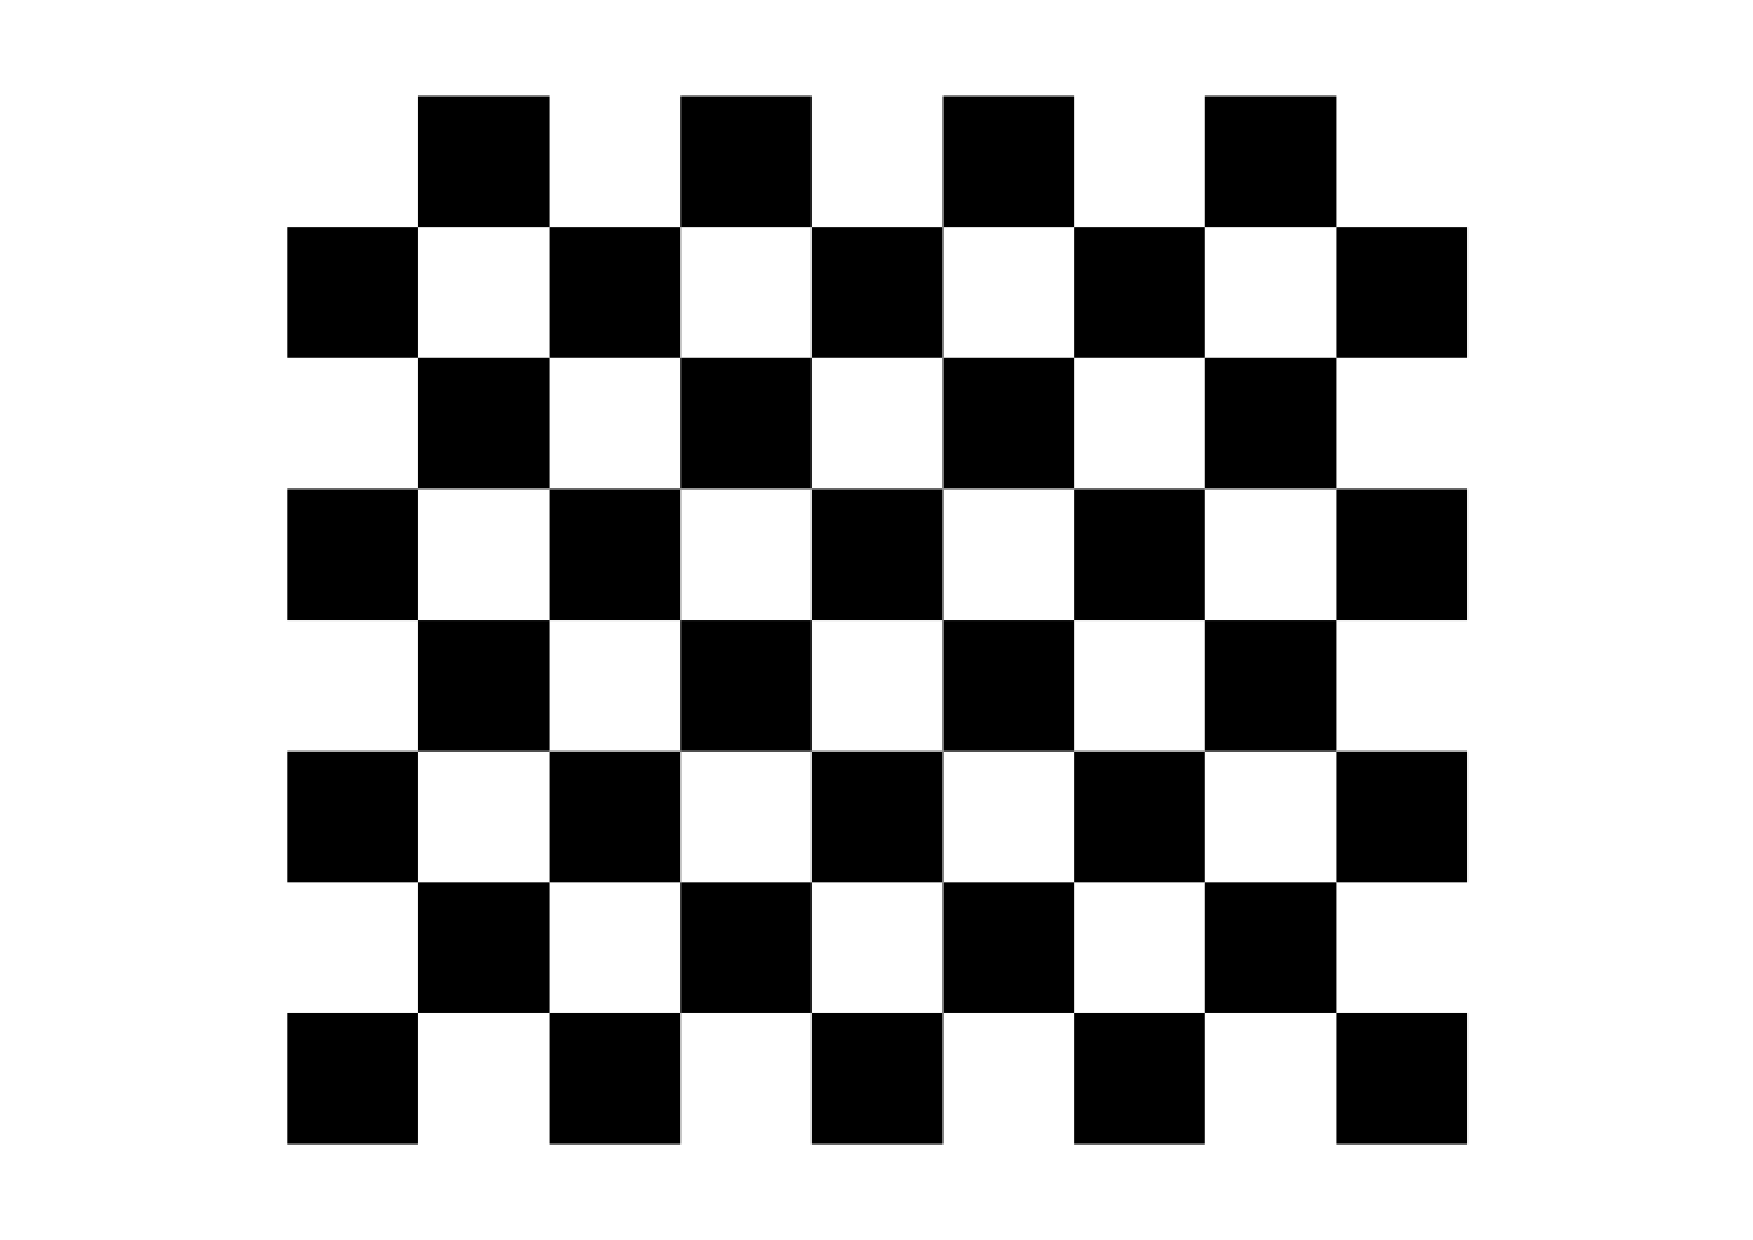
\includegraphics[width=0.8\linewidth]{img/chessboard/7x8chessboard}
	\caption{Example of $7\times8$ chessboard used for the calibration}
	\label{fig:chessboard}
\end{figure}

\subsection{How many images?} 

Now we know that, we can use a chessboard to calibrate the cameras. However,
the question of how many images are needed for the calibration remains. We
discuss only the images where the full chessboard is found. For enough
information from each image, we need a chessboard with at least $3\times3$
inner corners. It is better to have a chessboard with even, and odd dimension
(for example 7$\times$ 8 inner corners) since it has only one symmetry axis,
and the pose of the object can be detected correctly. It is important that the
chessboard indeed has squares, not rectangles (so it is better to check it
after printing). A bigger chessboard is easier to recognize, so we recommend at
least format A4.

We need only one image for computing the distortion coefficients. However, for
the camera matrix, we need at least two images. For stereo calibration, we need at
least one pair of images of the chessboard.

We know the minimum number of images needed for calibration. On the other hand,
we use more images for the robustness of the algorithm. We need a "rich" set of
views. Therefore it is important to move the chessboard between snapshots. With
more provided information to the algorithm, it compensates the errors in the
measurements (like a wrongly detected chessboard in one of the images).
Therefore also the computation time increases. Since it is enough for a given
setup of the cameras to perform a calibration only once and then use results
from it again, we recommend to do the calibration on more images and wait a
little bit longer for the results. 
